\documentclass[twocolumn, a4paper]{article}
\usepackage{graphicx}
\usepackage{hyperref}
\usepackage{listings}

\begin{document}
\title{Exponential function}
\author{Christiane Rahbek}
\date{\today}

\maketitle

\begin{abstract}
This is a short report on the exponential function, and how we can make a good approximation of the function.
\end{abstract}

\section{Introduction of the exponential function}
The exponential function is one of the most important functions in both mathematics and in physics. It can be defined in several different ways, but we will use the following definition:

\begin{equation} \label{eq:exp}
	\exp(x) = \sum_{k = 0}^{\infty} \frac{x^k}{k!} = 1 + x + \frac{x^2}{2} + \frac{x^3}{6} + \frac{x^4}{24} + \cdots
\end{equation}

The equation can be found with further details on Wikipedia \footnote{\url{https://en.wikipedia.org/wiki/Exponential_function}}

\section{Implementation}

There are 3 cases in the implementation. Fist have have the senario where $x < 0$.
Here we will return $\frac{1}{\exp{-x}}$, which is part of the definition of the exponential function. \\
Then we have the senario where $x > \frac{1.0}{8}$, where the following will be returned: $Pow(exp(x/2), 2)$.
This is actually not a nessesary implementation, but a very smart one. As we will see in a moment the last senario last thing we can return is an approximation of the exponential function, which means that it will only be valid up to a certain digit. This validity will quickly fall for big numbers of x, and therefore we use that

\begin{equation}
 x^a = \left(x^{\frac{a}{2}}\right)^2
\end{equation}

This will give us an overall greater pression on the digits of the exponential function. \\

The final implementation is just the taking eq. \ref{eq:exp} and instead of summning up to infinity there has been summed up to $k = 10$.

\section{How it works in practice}

\begin{figure} \label{fig:exp_dirty}
	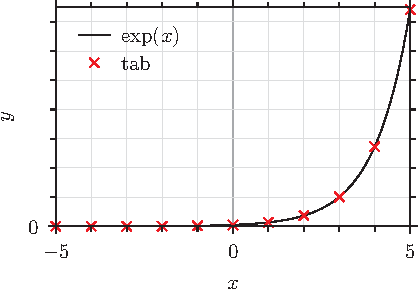
\includegraphics{exp_pyx.pdf}
	\caption{A plot of the "quick-and-dirty" implementation of the exponential function. Along with the plot of the function some values of the actual exponential function has been plotted.}
\end{figure}

Here we try to plot the function. It can be seen in fig. \ref{fig:exp_dirty}.

\end{document}
